% COS10022 Assignment 1 -- workflow explained (study companion, printable)
% Build: pdflatex workflow_explained.tex  (run twice)
\documentclass[11pt,a4paper]{article}
\usepackage[margin=2.1cm]{geometry}
\usepackage[T1]{fontenc}
\usepackage{lmodern}
\usepackage{amsmath}
\usepackage{booktabs,tabularx,array,longtable}
\usepackage{enumitem}
\usepackage[dvipsnames]{xcolor}
\usepackage[most]{tcolorbox}
\usepackage{tikz}
\usetikzlibrary{positioning,arrows.meta,fit}
\usepackage{float}
\usepackage[hidelinks]{hyperref}
\usepackage{fancyhdr}

\setlist{itemsep=2pt,topsep=3pt}
\setlength{\parindent}{0pt}
\setlength{\parskip}{5pt}
\renewcommand{\arraystretch}{1.18}
\newcolumntype{L}{>{\raggedright\arraybackslash}X}

\pagestyle{fancy}\fancyhf{}
\lhead{\small COS10022 Assignment 1 --- Workflow explained}
\rhead{\small\thepage}
\renewcommand{\headrulewidth}{0.4pt}

\newtcolorbox{keypoint}[1][Key point]{colback=Blue!4,colframe=Blue!55!black,fonttitle=\bfseries,title={#1},breakable,boxrule=0.6pt}
\newtcolorbox{issue}[1][Issue encountered]{colback=Red!4,colframe=Red!55!black,fonttitle=\bfseries,title={#1},breakable,boxrule=0.6pt}
\newtcolorbox{rubricbox}[1]{colback=Green!5,colframe=Green!45!black,fonttitle=\bfseries,title={#1},breakable,boxrule=0.6pt}
\newcommand{\nd}[1]{\textsf{\textbf{#1}}}          % node name
\newcommand{\cd}[1]{\texttt{#1}}                     % code / value

\tikzset{
  kn/.style={draw,rounded corners=2pt,fill=gray!8,minimum height=8mm,minimum width=25mm,
             align=center,font=\scriptsize\sffamily},
  data/.style={kn,fill=Goldenrod!25},
  model/.style={kn,fill=Blue!10},
  eval/.style={kn,fill=Green!12},
  arr/.style={-{Stealth[length=2mm]},thick},
  lab/.style={font=\scriptsize\itshape,fill=white,inner sep=1pt}
}

\begin{document}

%======================================================================
\begin{titlepage}
\centering
\vspace*{3cm}
{\LARGE\bfseries COS10022 Data Science Principles\par}
\vspace{4mm}
{\Large Assignment 1 --- Predictive Model Creation and Evaluation\par}
\vspace{1.2cm}
{\huge\bfseries The Workflow Explained\par}
\vspace{4mm}
{\large Design, every node, data decisions, results, insights,\\ troubleshooting and exploration\par}
\vspace{2cm}
\begin{minipage}{0.82\linewidth}
\begin{keypoint}[About this document]
A study companion for the KNIME workflow \cd{COS10022\_A1\_Workflow}, prepared with AI assistance
(Claude). The numbers are from the executed run of 10 October 2026, seed 2026, checked
independently by \cd{verify\_outputs.py} (result: PASS).\\[3pt]
Use it to understand the work and to plan your report. Declare it in the genAI appendix, and write
the report in your own words: Turnitin limits any single source to 5\%, and your video has to
explain the same reasoning naturally.
\end{keypoint}
\end{minipage}
\vfill
{\small Sections follow the marking rubric. Section~\ref{sec:rubric} maps each criterion to the pages that support it.}
\end{titlepage}

\tableofcontents
\newpage

%======================================================================
\section{What was built}
\begin{itemize}
  \item \textbf{One KNIME workflow, 28 nodes}, covering both tasks. Task~1 trains a logistic regression on
        \cd{accident\_2025\_train2\_73.csv} and tests it on \cd{accident\_2025\_test2\_73.txt}. Task~2 reads all four
        CSV files, builds a balanced 700-row training set and a 500-row test set, and compares logistic
        regression, Naïve Bayes and Random Forest on identical data.
  \item \textbf{Self-contained and portable}: the five input files are stored inside the workflow
        (\cd{data/src/}). Every reader and writer uses \emph{Relative to: Current workflow data area}, so the
        workflow runs unchanged on any computer. Outputs are written to \cd{data/output/}.
  \item \textbf{Reproducible}: every random step (Partitioning, Shuffle, Random Forest) uses seed 2026, so a re-run gives
        identical results. The brief gives no mark if the re-run differs from the report.
  \item \textbf{Independently verified}: a separate Python script re-reads KNIME's output files and checks row counts,
        class balance, shuffling and the absence of extra columns. It also reproduces the Task~1 result
        exactly with a different implementation of logistic regression.
  \item \textbf{Submission package}: \cd{COS10022\_A1\_submission.zip} holds the executed workflow (\cd{.knwf}), the
        input files (\cd{src/}), the output files (\cd{output/}) and run instructions. The video still has to be added.
\end{itemize}

%======================================================================
\section{Understanding the data and the cleaning decisions}

\subsection{What the data looks like}
\begin{tabularx}{\linewidth}{@{}lL@{}}
\toprule
Attribute & Type and range \\ \midrule
Age & integer, 18--69 \\
Gender & nominal: Male / Female \\
Speed\_of\_Impact & integer, 20--119 \\
Helmet\_Used, Seatbelt\_Used & nominal: Yes / No \\
Survived (\emph{target}) & nominal: Yes / No \\ \bottomrule
\end{tabularx}

\begin{tabularx}{\linewidth}{@{}lrrL@{}}
\toprule
File & Rows & Format & Note \\ \midrule
\cd{accident\_2025\_train1\_73.csv} & 420 & comma & \\
\cd{accident\_2025\_train2\_73.csv} & 420 & comma & Task 1 training set \\
\cd{accident\_2025\_test1\_73.csv}  & 180 & comma & \\
\cd{accident\_2025\_test2\_73.csv}  & 180 & comma & same data as the .txt \\
\cd{accident\_2025\_test2\_73.txt}  & 180 & \textbf{tab}, CRLF & Task 1 test set \\ \bottomrule
\end{tabularx}

\subsection{Five facts found during exploration}
\begin{enumerate}
  \item \textbf{The four CSVs are two different 70/30 splits of the same 600 records.} train1+test1 and
        train2+test2 contain the same records. Reading all four gives 1,200 rows, but only \textbf{599 are unique}:
        every record appears twice.
  \item \textbf{Every file is sorted}: all ``No'' rows first, then all ``Yes'', each in descending speed.
  \item \textbf{Class imbalance}: across the four CSVs, 378 Yes (31.5\%) and 822 No (68.5\%).
  \item \textbf{A hard threshold}: nobody survives at a speed of 90 or more; below 90, about 45\% survive.
  \item \textbf{Only 189 unique ``Yes'' records exist} (and 410 unique ``No'').
\end{enumerate}

\subsection{Cleaning decisions --- and why ``no cleaning'' was the right answer}
The brief states the data is ``cleaned and organised with no missing data''. This was checked rather than
assumed: no missing values, no out-of-range numbers, no misspelt categories. Each preprocessing step was then
considered and deliberately rejected:

\begin{tabularx}{\linewidth}{@{}p{3.6cm}L@{}}
\toprule
Decision & Justification \\ \midrule
No missing-value handling & There are none, confirmed per column. \\
No normalisation & IRLS logistic regression does not need scaled inputs to converge; scaling would only change
  how the coefficients read. Naïve Bayes fits a distribution per attribute, and Random Forest only compares split
  thresholds, so neither is affected by scale. \\
\textbf{No duplicate removal} & Removing duplicates leaves \textbf{189 unique survivors, but the brief requires 350}.
  The task cannot be completed on de-duplicated data. The duplicates were kept as the brief requires, and their
  effect (train/test leakage) was \emph{measured} instead (Section~\ref{sec:insights}). \\
All five attributes used & The brief: ``feeding all attributes into the model''. \\
Survived kept nominal & Classifiers need a nominal target; a 0/1 number would be treated as a regression target. \\
Age and Speed kept numeric & They are measurements; logistic regression fits one slope per numeric attribute. \\
\bottomrule
\end{tabularx}

\begin{keypoint}[Why these facts drive the design]
Sorted files mean random sampling and shuffling are essential. The imbalance means accuracy is a misleading
metric. The duplicates mean the test set overlaps the training set. The speed threshold explains why a tree-based
model has an advantage. Each later design choice comes back to one of these facts.
\end{keypoint}

%======================================================================
\section{Workflow design}

\subsection{Design principles}
The workflow follows Phase~4 of the Data Analytics Lifecycle (Model Building): prepare training and test data,
build models, evaluate them. Six principles guided the layout:
\begin{enumerate}
  \item \textbf{Separate stages}: read $\rightarrow$ prepare $\rightarrow$ learn $\rightarrow$ predict $\rightarrow$ evaluate,
        left to right, with no loops, so every number can be traced back to its source.
  \item \textbf{Verify each stage} before the next uses it (row counts, column types, class counts), so loading
        errors cannot quietly reach the models.
  \item \textbf{One training set and one test set feed all three models}, so differences in results come from the
        algorithms, not from the data.
  \item \textbf{No test data ever reaches a learner}: the test Shuffle connects only to predictors.
  \item \textbf{Reproducibility}: a fixed seed on every random node.
  \item \textbf{Portability and evidence}: relative paths, and CSV Writers that save the intermediate sets and all
        predictions as output files.
\end{enumerate}

\subsection{Task 1 layout}
\begin{figure}[H]\centering
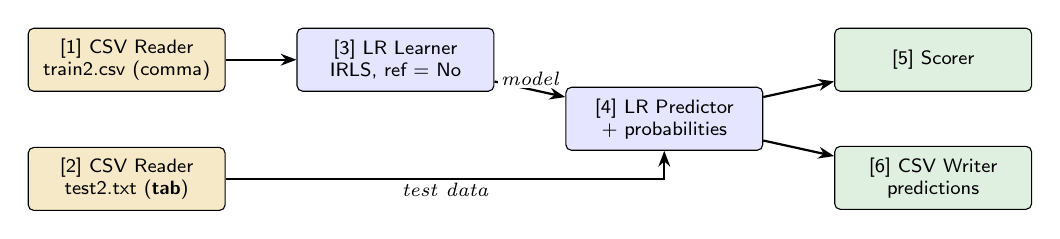
\begin{tikzpicture}[node distance=7mm and 9mm]
\node[data] (r1) {[1] CSV Reader\\train2.csv (comma)};
\node[data,below=of r1] (r2) {[2] CSV Reader\\test2.txt (\textbf{tab})};
\node[model,right=of r1] (l) {[3] LR Learner\\IRLS, ref = No};
\node[model,right=of l, yshift=-7.5mm] (p) {[4] LR Predictor\\+ probabilities};
\node[eval,right=of p, yshift=7.5mm] (s) {[5] Scorer};
\node[eval,right=of p, yshift=-7.5mm] (w) {[6] CSV Writer\\predictions};
\draw[arr] (r1)--(l); \draw[arr] (l)--node[lab,above]{model}(p); \draw[arr] (r2)-|node[lab,pos=0.25,below]{test data}(p);
\draw[arr] (p)--(s); \draw[arr] (p)--(w);
\end{tikzpicture}
\caption{Task 1: one learner, one predictor, evaluated on the specified test file.}
\end{figure}

\subsection{Task 2 layout}
\begin{figure}[H]\centering
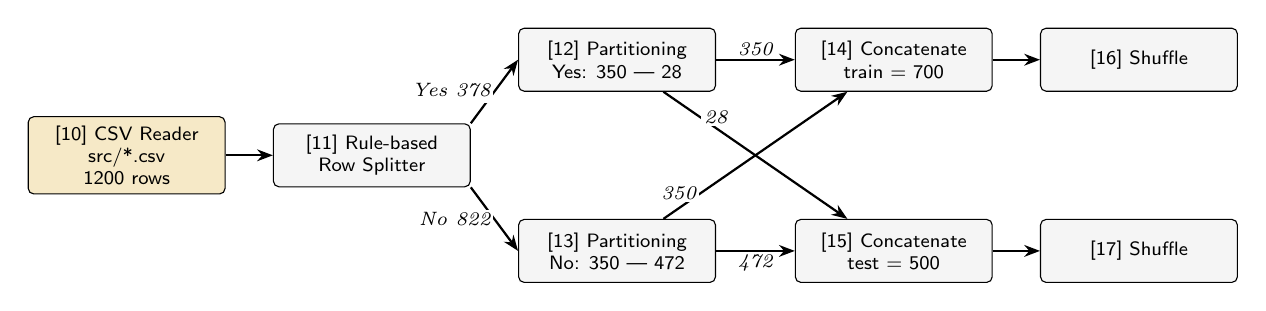
\begin{tikzpicture}[node distance=6mm and 6mm]
\node[data] (r) {[10] CSV Reader\\src/*.csv\\1200 rows};
\node[kn,right=of r] (sp) {[11] Rule-based\\Row Splitter};
\node[kn,above right=4mm and 6mm of sp] (py) {[12] Partitioning\\Yes: 350 | 28};
\node[kn,below right=4mm and 6mm of sp] (pn) {[13] Partitioning\\No: 350 | 472};
\node[kn,right=10mm of py] (ct) {[14] Concatenate\\train = 700};
\node[kn,right=10mm of pn] (ce) {[15] Concatenate\\test = 500};
\node[kn,right=of ct] (st) {[16] Shuffle};
\node[kn,right=of ce] (se) {[17] Shuffle};
\draw[arr] (r)--(sp);
\draw[arr] (sp.north east)--node[lab,left]{Yes 378}(py.west);
\draw[arr] (sp.south east)--node[lab,left]{No 822}(pn.west);
\draw[arr] (py)--node[lab,above]{350}(ct); \draw[arr] (pn)--node[lab,pos=0.2,left]{350}(ct);
\draw[arr] (py)--node[lab,pos=0.2,right]{28}(ce); \draw[arr] (pn)--node[lab,below]{472}(ce);
\draw[arr] (ct)--(st); \draw[arr] (ce)--(se);
\end{tikzpicture}
\vspace{9mm}
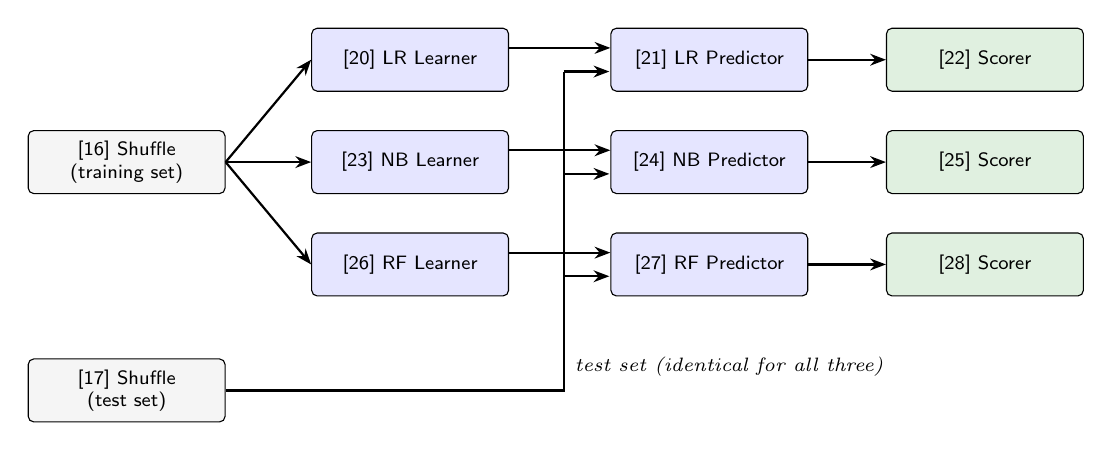
\begin{tikzpicture}
\node[kn] (st) at (0,0) {[16] Shuffle\\(training set)};
\node[kn] (se) at (0,-2.9) {[17] Shuffle\\(test set)};
\node[model] (l1) at (3.6,1.3)  {[20] LR Learner};
\node[model] (l2) at (3.6,0)    {[23] NB Learner};
\node[model] (l3) at (3.6,-1.3) {[26] RF Learner};
\node[model] (p1) at (7.4,1.3)  {[21] LR Predictor};
\node[model] (p2) at (7.4,0)    {[24] NB Predictor};
\node[model] (p3) at (7.4,-1.3) {[27] RF Predictor};
\node[eval]  (s1) at (10.9,1.3)  {[22] Scorer};
\node[eval]  (s2) at (10.9,0)    {[25] Scorer};
\node[eval]  (s3) at (10.9,-1.3) {[28] Scorer};
\foreach \i in {1,2,3}{
  \draw[arr] (st.east) -- (l\i.west);
  \draw[arr] ([yshift=1.5mm]l\i.east) -- ([yshift=1.5mm]p\i.west);
  \draw[arr] (p\i) -- (s\i);
}
\draw[thick] (se.east) -- (5.55,-2.9) -- (5.55,1.15);
\foreach \y in {1.15,-0.15,-1.45}{\draw[arr] (5.55,\y) -- (6.13,\y);}
\node[lab,anchor=west] at (5.65,-2.6) {test set (identical for all three)};
\end{tikzpicture}
\caption{Task 2: class-wise sampling builds one training and one test set, shared by all three models.
CSV Writers (not drawn) save the 700/500 sets and every model's predictions.}
\end{figure}

%======================================================================
\section{Task 1 --- node by node}

\subsection*{[1] CSV Reader --- training file}
\begin{tabularx}{\linewidth}{@{}p{3.4cm}p{3.6cm}L@{}}
\toprule Setting & Value & Reason \\ \midrule
File & \cd{src/accident\_2025\_}\newline\cd{train2\_73.csv} & the training file named in the brief \\
Path mode & relative to workflow data area & runs on any computer \\
Delimiter / header & comma / first row & the file's actual format \\
Column types & auto-detected & Age, Speed integer; others string \\
Append path column & off & a path column would become a feature \\ \bottomrule
\end{tabularx}
\textit{Check}: 420 rows, 6 columns.

\subsection*{[2] CSV Reader --- test file (the loading problem)}
\begin{issue}[Issue encountered: the test file is tab-separated]
\textbf{Symptom}: with the default comma delimiter, every line of \cd{accident\_2025\_test2\_73.txt} lands in a single
column, and the predictor cannot find Age, Speed and the other attributes.\\
\textbf{Cause}: the .txt uses \textbf{tab} separators and Windows (CRLF) line endings, while every other file
uses commas.\\
\textbf{Fix}: column delimiter set to \textbf{Tab} (\cd{\textbackslash t}). The line-break row delimiter handles CRLF.\\
\textbf{Confirmation}: 180 rows, 6 columns, \emph{with the same names and types as the training file}. The predictor
requires the test table to match the columns the model was trained on.\\
\textbf{Why not use test2.csv instead?} It has the same data, but the brief names the .txt.
\end{issue}

\subsection*{[3] Logistic Regression Learner}
\textbf{Theory.} A linear score $z = w_0 + w_1x_1 + \dots + w_kx_k$ is turned into a probability by the sigmoid,
$P(\text{Yes}) = 1/(1+e^{-z})$. Equivalently, $\log\frac{p}{1-p} = z$: each coefficient is the change in log-odds per
unit of its input, and $e^{w}$ is the odds ratio. Nominal inputs are dummy-coded against a base level. The decision
boundary is linear, so a sharp cut-off (speed $\ge 90$) can only be approximated by a smooth slope.

\begin{tabularx}{\linewidth}{@{}p{3.4cm}p{3.0cm}L@{}}
\toprule Setting & Value & Reason \\ \midrule
Target & Survived & the label to predict \\
Features & all five & brief: all attributes \\
Reference category & \textbf{No} & coefficients then describe the odds of \emph{surviving}; a positive sign means ``raises survival odds'' \\
Solver & \textbf{IRLS} & iteratively reweighted least squares gives the exact maximum-likelihood fit and is
  deterministic; ideal for 420 rows. SAG (stochastic average gradient) is approximate and depends on epochs, step
  size and seed; it is meant for large data. \\
Max epochs / $\epsilon$ & 100 / $10^{-5}$ & stopping rules; IRLS converges in a few iterations \\
Coefficient statistics & on & standard errors and p-values show which features matter \\
Seed & 2026 & only SAG uses it; fixed for consistency \\ \bottomrule
\end{tabularx}

\subsection*{[4] Logistic Regression Predictor}
Inputs: port 1 = model from [3], port 2 = test data from [2]. Class probabilities P(Yes)/P(No) appended, so
confidence can be discussed, not just labels.

\subsection*{[5] Scorer and [6] CSV Writer}
The Scorer compares \cd{Survived} (actual) with \cd{Prediction (Survived)} and reports the confusion matrix, accuracy,
Cohen's kappa and per-class recall, precision, specificity and F-measure. The writer saves
\cd{output/task1\_LR\_predictions.csv}, overwriting on re-run so execution never fails.

%======================================================================
\section{Task 2 --- data preparation, node by node}

\subsection*{[10] CSV Reader --- reading every CSV without touching \cd{src}}
\begin{tabularx}{\linewidth}{@{}p{3.4cm}p{3.4cm}L@{}}
\toprule Setting & Value & Reason \\ \midrule
Mode & \textbf{Files in folder}: \cd{src} & one node reads every file; the folder itself is never changed \\
File filter & extension = \cd{csv} & includes the four CSVs, excludes the .txt (which is not a CSV) \\
Prepend file index to RowID & on & each file numbers its rows from Row0; without the prefix the RowIDs collide \\
Append path column & \textbf{off} & otherwise a ``Path'' column becomes a feature that reveals which file a row came from \\
Fail on differing specs & on & a file with a different structure stops the node instead of corrupting data \\ \bottomrule
\end{tabularx}
\textit{Check}: 1,200 rows (4 files), 6 columns, no Path column.

\subsection*{[11] Rule-based Row Splitter}
\textbf{Rule}: \cd{\$Survived\$ = "Yes" => TRUE}. Rows where it is TRUE go to the top port, all others to the bottom.
\begin{itemize}
  \item \cd{\$Survived\$} refers to the column; \cd{"Yes"} is a text constant; \cd{=>} gives the outcome.
  \item \textbf{Result}: top = 378 Yes, bottom = 822 No; $378 + 822 = 1200$ confirms no row was lost.
  \item \textbf{Why split by class first}: so exactly 350 can be drawn from \emph{each} class. One random split of the
        whole table would give an unpredictable class mix.
\end{itemize}
\begin{issue}[How the splitter connects to the issues]
\textbf{Sorted data}: each output is a block of rows in file order (descending speed), so the next node must sample
randomly.
\textbf{Duplicates}: both copies of each record land in the same output, which is where the later train/test
overlap starts.
\textbf{Exact text match}: \cd{"yes"} or \cd{"Yes "} would send every row to the bottom port. Checking 378/822 proves the
rule works.
\end{issue}

\subsection*{Workflow Coach --- finding the partitioning node}
The brief requires the Workflow Coach to be used \emph{at one of the splitter's outputs} and the prompt to be
reported. Click an output port of [11], ask for a node that splits a table into an exact number of rows, and record the
exact wording and the suggestions (screenshot). A prompt following the week~2 structure states the
\emph{task} (split into two groups), the \emph{constraint} (exactly 350 rows, the rest in the other group) and the
\emph{context} (the input is one class from the splitter). Justify choosing \nd{Partitioning} over alternatives such as
Row Sampling (which discards the remainder) or Row Splitter (rule-based, not count-based).

\subsection*{[12] and [13] Partitioning}
\begin{tabularx}{\linewidth}{@{}p{3.4cm}p{3.0cm}L@{}}
\toprule Setting & Value & Reason \\ \midrule
Mode & \textbf{Absolute, 350} & the brief requires \emph{exactly} 350; a percentage cannot guarantee an exact count \\
Sampling & \textbf{Draw randomly} & the input is sorted by speed, so ``take from top'' would select the 350 fastest crashes, a biased sample \\
Seed & 2026 & the same 350 rows on every run \\ \bottomrule
\end{tabularx}
Yes branch [12]: top = 350 (training), bottom = 28 (test). No branch [13]: top = 350, bottom = 472.

\subsection*{[14] and [15] Concatenate}
[14] stacks the two 350-row top outputs into the \textbf{700-row training set} (balanced 50/50). [15] stacks the
remainders into the \textbf{500-row test set} (28 Yes, 472 No). Settings: union of columns; duplicate RowIDs get a
suffix instead of failing. None occur here because of the file-index prefix, but this is the safe setting.

\subsection*{[16] and [17] Shuffle}
After concatenation, the rows sit in blocks (all Yes, then all No). Shuffling removes that order, which matters for
learners that process rows in sequence or in batches. The brief requires both sets to be shuffled. Seed 2026 keeps the
order reproducible.

\subsection*{[18] and [19] CSV Writers}
Save \cd{task2\_train\_700.csv} and \cd{task2\_test\_500.csv}: evidence of the exact counts, and the
intermediate files the brief asks for.

%======================================================================
\section{Model construction}
All three learners take the same training table [16]; all three predictors take the same test table [17].

\subsection*{[20]--[22] Logistic Regression}
Same configuration as Task~1 (Section~4), so the two logistic regression results can be compared directly.

\subsection*{[23]--[25] Naïve Bayes}
\textbf{Theory.} $P(c \mid a_1,\dots,a_m) \propto P(c)\prod_j P(a_j \mid c)$. ``Naïve'' means the attributes are assumed
independent given the class. Nominal attributes use frequency tables; numeric attributes (Age, Speed) use a
Gaussian per class. $P(c)$, the \textbf{prior}, is learned from the training class proportions: here 50/50 by
construction.\\
\textbf{Settings}: class column Survived; minimum standard deviation $10^{-4}$ (avoids division by zero); maximum 20
distinct nominal values (each attribute has 2); predictor appends class probabilities.

\subsection*{[26]--[28] Random Forest}
\textbf{Theory.} An ensemble of decision trees. Each tree is trained on a bootstrap sample (rows drawn with
replacement) and considers a random subset of attributes at each split; the forest predicts by majority vote. Trees
split on thresholds, so ``Speed $< 90$'' can be learnt directly. Deep trees can memorise individual records.

\begin{tabularx}{\linewidth}{@{}p{3.4cm}p{3.4cm}L@{}}
\toprule Setting & Value & Reason \\ \midrule
Number of trees & 100 & KNIME default; ample for five attributes \\
Split criterion & Information Gain Ratio & default; corrects information gain's bias towards attributes with many values \\
Attribute sampling & square root ($\sqrt5 \approx 2$) & different trees see different attributes, which strengthens the ensemble \\
Row sampling & bootstrap, 100\% & each tree learns from a different resample \\
Tree depth & unlimited & default (an overfitting risk discussed later) \\
Seed & \textbf{2026} & otherwise each run grows different trees \\ \bottomrule
\end{tabularx}

%======================================================================
\section{Results}

\subsection{Task 1}
Training: 300 No / 120 Yes. Test: 111 No / 69 Yes.

\begin{center}
\begin{tabular}{@{}lcc@{}}\toprule
 & Predicted No & Predicted Yes \\ \midrule
Actual No  & 92 & 19 \\
Actual Yes & 45 & 24 \\ \bottomrule
\end{tabular}\qquad
\begin{tabular}{@{}lr@{}}\toprule
Accuracy & 0.644 \\ Always-``No'' baseline & 0.617 \\ Cohen's kappa & 0.190 \\
Recall (Yes) & 0.348 \\ Precision (Yes) & 0.558 \\ Specificity & 0.829 \\ \bottomrule
\end{tabular}
\end{center}

Logistic regression beats guessing ``No'' by only 2.7 percentage points and misses 65\% of survivors. It leans
towards ``No'' because 71\% of its training rows were ``No''. This exact result was reproduced by an independent
implementation of unpenalised logistic regression.

\textbf{Coefficients} (read them from node [3]'s coefficient table; the independent check gives these signs and sizes):
Seatbelt $\approx +1.0$ (about $2.7\times$ the odds of surviving), Helmet $\approx +0.8$ ($\approx 2.2\times$),
Speed $\approx -0.035$ per km/h ($\approx 0.70\times$ the odds per extra 10\,km/h), Age $\approx 0$ (no effect).
These agree with common sense, which supports the model. Report which ones are statistically significant
(p-values).

\subsection{Task 2}
Training: 350 Yes / 350 No. Test: 28 Yes / 472 No.

\begin{table}[H]\centering\small
\begin{tabular}{@{}lrrrrrr@{}}\toprule
Model & Accuracy & Kappa & Recall Yes & Precision Yes & F$_1$ Yes & Specificity \\ \midrule
Always ``No'' & \textbf{0.944} & 0 & 0 & -- & -- & 1 \\
Logistic Regression & 0.706 & 0.131 & 0.714 & 0.126 & 0.214 & 0.706 \\
Naïve Bayes & 0.674 & 0.120 & 0.750 & 0.119 & 0.205 & 0.669 \\
Random Forest & \textbf{0.752} & \textbf{0.222} & \textbf{0.929} & \textbf{0.176} & \textbf{0.295} & \textbf{0.742} \\ \bottomrule
\end{tabular}
\caption{Task 2 test-set results (positive class = Yes). Check them against your Scorer nodes.}
\end{table}

\begin{center}\small
\begin{tabular}{@{}lcccc@{}}\toprule
Model & TN & FP & FN & TP \\ \midrule
LR & 333 & 139 & 8 & 20 \\ NB & 316 & 156 & 7 & 21 \\ RF & 350 & 122 & 2 & 26 \\ \bottomrule
\end{tabular}
\end{center}

%======================================================================
\section{Comparison and insights}\label{sec:insights}

\begin{enumerate}[leftmargin=*]
\item \textbf{Every model is less accurate than always answering ``No''.} On a test set that is 94.4\% ``No'',
  accuracy mostly measures agreement with the majority class. Kappa, F$_1$, and recall and precision for ``Yes'' show
  usefulness. The week~4 lecture makes the same point: accuracy alone does not establish a good model, and which error
  matters (Type~I vs.\ Type~II) depends on the situation. For accident survival, missing a survivor and wrongly
  predicting survival have very different costs.

\item \textbf{The balanced training set shifts every model towards ``Yes''.} The models learnt in a 50/50 world and
  were tested in a 94/6 world. They find most survivors (recall 0.71--0.93), but at least 8 out of 10 of their
  ``survived'' predictions are wrong (precision 0.12--0.18). Naïve Bayes is affected directly through its prior
  $P(\text{Yes}) = 0.5$, where the test rate is $0.056$.

\item \textbf{The same algorithm, a different training mix: Task 1 vs.\ Task 2 logistic regression.} Recall rose from
  0.35 to 0.71, and precision fell from 0.56 to 0.13. Nothing changed except the class balance of the training data.
  That is the clearest evidence of the prior effect.

\item \textbf{Random Forest wins, for two different reasons.}
  \begin{itemize}
    \item \emph{It suits the shape of the data}: survival drops to zero above speed 90. A tree learns that threshold
      directly; logistic regression can only fit a smooth slope in log-odds, and Naïve Bayes models speed as a bell
      curve per class.
    \item \emph{Leakage}: 222 of the 500 test rows (44\%) are identical to a training row, because every record exists
      twice. Random Forest scores \textbf{0.793 on those rows and 0.719 on unseen rows}. Logistic regression (0.698 vs.\
      0.712) and Naïve Bayes (0.662 vs.\ 0.683) show no such gap, because they cannot memorise individual records.
      Part of Random Forest's lead is memorisation, and on genuinely unseen data it only roughly ties logistic
      regression.
  \end{itemize}

\item \textbf{The ``IID'' training set, examined critically.} The brief calls the 700-row set IID (independent and
  identically distributed). Its class mix (50/50) matches neither the source data (31.5\% Yes) nor the test set
  (5.6\% Yes), and 44\% of the test set duplicates it. The two sets are neither identically distributed nor
  independent. The design is good for learning what separates the classes, but it does not give an honest estimate of
  real-world performance.
\end{enumerate}

\begin{keypoint}[Suggestions]
\begin{itemize}
  \item Remove duplicates \emph{before} splitting. This would make the 350-per-class requirement impossible (189 unique
        survivors), so the sampling design itself would need to change, e.g.\ a stratified 70/30 split.
  \item Use k-fold cross-validation (X-Partitioner/X-Aggregator, week~4) rather than a single holdout split.
  \item Evaluate with kappa, F$_1$ or AUC, and choose the metric according to which error is more costly.
  \item Adjust the decision threshold, or correct the priors, to match the real-world class rate.
  \item Limit Random Forest depth to reduce memorisation; collect more informative attributes.
\end{itemize}
\end{keypoint}

%======================================================================
\section{Problem solving and troubleshooting}
Problems you are likely to meet when building this by hand, with symptoms and fixes:

\begin{longtable}{@{}p{4.1cm}p{5.3cm}p{6.2cm}@{}}
\toprule Problem & Symptom & Fix \\ \midrule\endhead
Tab-delimited .txt & test table has one column; predictor error & delimiter = Tab \\
Train/test types differ & predictor reports missing or mismatched columns & make both readers produce identical names and types \\
Folder reader includes the .txt & ``differing specs'' error or a garbage column & extension filter \cd{csv} \\
Path column left on & a ``Path'' feature appears in the models & turn off ``append path column'' \\
Four readers + Concatenate & duplicate RowID error & file-index prefix, or Concatenate ``append suffix'' \\
Relative (\%) partitioning & 349 or 351 rows instead of 350 & Absolute, 350 \\
``Take from top'' sampling & training set holds only high-speed crashes & Draw randomly \\
No seeds & numbers change each run; report no longer matches & seed on Partitioning, Shuffle, Random Forest \\
Splitter text typo (\cd{"yes"}) & all rows in one output & exact \cd{"Yes"}; check 378/822 \\
Concatenate inputs swapped & training set of 378 or 822 rows & top outputs $\rightarrow$ train, bottom outputs $\rightarrow$ test \\
Predictor ports swapped & cannot connect, or no prediction column & model $\rightarrow$ port 1, data $\rightarrow$ port 2 \\
Scorer columns wrong & empty or meaningless matrix & Survived vs.\ Prediction (Survived) \\
Target read as a number & learner refuses the target & keep Survived nominal \\
SAG solver & ``did not converge'' warning; results vary with seed & IRLS, or more epochs \\
Coefficient signs look backwards & ``seatbelt lowers survival?'' & check the reference category \\
Absolute file paths & fails on the tutor's computer & relative to workflow data area \\
Workflow Coach empty / K-AI unavailable & no suggestions & enable it in preferences and log in to KNIME Hub; K-AI has a monthly limit \\
Exporting without data & tutor's copy has no inputs or outputs & files in the data area; export the executed workflow \\
\bottomrule
\end{longtable}

%======================================================================
\section{Exploration and discovery in self-learning}
The Excellent band asks for independent exploration of tools \emph{and} concepts, discoveries about workflow design,
model behaviour and theory, experiments with multiple approaches, and critical reflection. Candidate explorations,
each with the question, the method and what it shows:

\begin{tabularx}{\linewidth}{@{}p{3.3cm}L@{}}
\toprule Exploration & Question, method, finding \\ \midrule
Leakage analysis & \emph{Does the test set overlap the training set?} Match test rows to training rows (Joiner on all
  columns). Finding: 222/500 overlap; Random Forest 0.79 on seen vs.\ 0.72 on unseen rows; logistic regression and
  Naïve Bayes show no gap. Shows memorisation and why test data must be independent. \\
De-duplication paradox & \emph{Can the task run on clean data?} Count unique records per class (Duplicate Row
  Filter + GroupBy). Finding: 189 unique survivors, below the 350 required. The design depends on duplicates. \\
Speed threshold & \emph{Which attribute drives survival?} Survival rate by speed band (Binner + GroupBy, or a bar
  chart). Finding: 0\% above 90. Links data understanding to model choice. \\
Training mix effect & \emph{Why does the same algorithm behave differently?} Compare Task~1 and Task~2 logistic
  regression. Finding: recall 0.35 $\rightarrow$ 0.71, precision 0.56 $\rightarrow$ 0.13. The prior effect. \\
Seed sensitivity & \emph{How reliable is one split?} Re-run Task~2 with 2--3 seeds and report the spread. Motivates
  cross-validation. \\
IRLS vs.\ SAG & \emph{Does the optimiser matter?} Compare coefficients and accuracy. Exact vs.\ approximate
  optimisation. \\
Limiting tree depth & \emph{Is Random Forest memorising?} Limit depth and compare seen vs.\ unseen accuracy. \\
\bottomrule
\end{tabularx}

\textbf{Writing the reflection.} Be specific: what surprised you (models below the always-``No'' baseline; Random
Forest's lead partly from memorisation; a ``clean'' dataset that cannot be de-duplicated), which theory explained it
(priors, leakage, linear vs.\ threshold decision boundaries), and what you would do differently (de-duplicate
first, cross-validate, choose metrics by error cost).

%======================================================================
\section{Rubric map}\label{sec:rubric}
\begin{tabularx}{\linewidth}{@{}p{4.6cm}rL@{}}
\toprule Criterion & Weight & Covered in \\ \midrule
Understanding of workflow design & 5\% & Section 3 (principles, diagrams) \\
Detailed node configuration & 15\% & Sections 4, 5, 6 (every setting with its reason) \\
Data loading and preprocessing & 10\% & Section 2, node [2] issue, node [10] \\
Rule-based Row Splitter & 5\% & node [11] and its issue box \\
Dataset partitioning & 10\% & nodes [12]--[17] \\
Workflow Coach and node selection & 5\% & Workflow Coach subsection (your own prompt and screenshot) \\
Model construction & 5\% & Section 6 \\
Model evaluation and results & 10\% & Section 7 \\
Comparison and insights & 10\% & Section 8 \\
Problem solving and troubleshooting & 5\% & node [2] and [11] issues; Section 9 \\
Report quality and presentation & 10\% & numbered, captioned figures and tables; consistent terms \\
Exploration and self-learning & 10\% & Section 10 \\ \bottomrule
\end{tabularx}

\subsection*{Before you submit}
\begin{itemize}
  \item Header on page 1: name, student ID, unit code, class, tutor. At most 10 pages. Questions in the brief's order.
  \item Your own Workflow Coach prompt and screenshot; your own screenshots of every node dialog and Scorer.
  \item Re-import the submitted \cd{.knwf}, run it, and confirm it matches the report.
  \item Video inside the zip. GenAI declaration appendix completed. Turnitin below 25\% overall and below 5\% per source.
\end{itemize}

%======================================================================
\appendix
\section{Metric formulas}
With positive class = Yes:
\begin{align*}
\text{Accuracy} &= \tfrac{TP+TN}{TP+TN+FP+FN} &
\text{Recall} &= \tfrac{TP}{TP+FN} &
\text{Precision} &= \tfrac{TP}{TP+FP} \\
\text{Specificity} &= \tfrac{TN}{TN+FP} &
F_1 &= \tfrac{2PR}{P+R} &
\kappa &= \tfrac{p_o-p_e}{1-p_e}
\end{align*}
where $p_o$ is the observed accuracy and $p_e$ the accuracy expected by chance from the row and column totals.
Worked example (Random Forest): $p_o = 0.752$; $p_e = 0.056 \times 0.296 + 0.944 \times 0.704 = 0.681$;
$\kappa = (0.752 - 0.681)/(1 - 0.681) = 0.222$.

\section{Glossary}
\begin{tabularx}{\linewidth}{@{}p{3.6cm}L@{}}
\toprule
Holdout split & dividing data once into training and test sets \\
IID & independent and identically distributed: each record drawn independently from the same distribution \\
Data leakage & information from the test set present in training, inflating test scores \\
Prior & a class's probability before seeing the attributes; learnt from the training proportions \\
Bootstrap sample & a resample of the same size drawn with replacement \\
Reference category & the class the logistic regression coefficients are measured against \\
Majority-class baseline & the score of always predicting the most common class \\
Cohen's kappa & agreement between predictions and truth beyond what chance would give \\ \bottomrule
\end{tabularx}

\end{document}
